\documentclass[12pt,a4paper]{scrartcl}
\usepackage[utf8]{inputenc}
\usepackage[ngerman]{babel}
\usepackage{amsmath}
\usepackage{amsfonts}
\usepackage{amssymb}
\usepackage{blindtext}
\usepackage{graphicx}
\usepackage[hidelinks]{hyperref}


\usepackage[left=2.5cm,right=1.5cm,top=2cm,bottom=2.8cm]{geometry}


\usepackage{fancyhdr}
\pagestyle{fancy}

\begin{document}
\begin{titlepage}
\begin{center}

\vspace*{3cm}
\textbf{\huge{Projektarbeit}}\\
\vspace*{2cm}
\textbf{\large{Entwicklung eines 2D-Spiels mit SFML}}\\
\vspace*{5cm}
Gabriel Gavrilas, G3C\\
Jan Kunzmann, G3C\\
Patrick Eigensatz, G3C
\end{center}
\end{titlepage}




\newpage

\setcounter{page}{1}
\section*{Vorwort}
\blindtext[1]

\newpage


\tableofcontents

\newpage


\section{Motivation}
\subsection{Warum ein 2D-Spiel?}
Als wir uns für ein Projektthema entscheiden mussten, haben
wir uns die Entscheidung schwer gemacht. Aus 5 verschiedenen
Bereichen, für die wir uns alle sehr interessierten, entschieden wir uns für die
eines Computerspieles.

\subsection{Warum C++ und SFML?}
Um die Sache für uns attraktiv zu machen,
wählten wir bewusst eine Programmiersprache, die noch nicht
alle von uns beherrschten. Natürlich hätten wir genau so gut
SDL oder direkt das darunterliegende OpenGL verwenden können. OpenGL
schied aus, da der Aufwand bereits ein einfaches 2D-Spiel zu realisieren,
schlichtweg nicht möglich gewesen wäre. SDL war unser Favorit, bis wir
SFML entdeckten. Ganz im Gegensatz zu SDL schien SFML für C++ ausgerichtet
zu sein. So wurden Klassen anstatt Strukturen verwendet, was den (für den
Anfang komplizierten) Umgang mit Zeigern reduzierte. Ausserdem besitzen die
Klassen eigene Konstruktoren, bzw. Destruktoren, was das Initialisieren
oder das freigeben von Speicher überflüssig macht. Davon erhofften wir uns
weniger Speicherzugriffsfehler und ein schnelleres programmieren. SFML
überzeugte uns schlussendlich, als wir die in der offiziellen Dokumentation
gezeigten Beispielprogramme angeschaut haben.

\section{Vorgehen}
Am Anfang stand ganz klar die Ideenfindung auf dem Programm. Es war uns wichtig,
eine Spielidee zu finden, an der ein Spieler später auch Spass haben würde,
und wir das Spiel je nach zeitlichen Kapazitäten auch etwas erweitern könnten.
Diese drei Fragen halfen uns:
\begin{enumerate}
\item Würdest du das Spiel spielen?
\item Ist das Spiel technisch überhaupt realisierbar?
\item Ist das Spiel erweiterbar?
\end{enumerate}
Der Ideenfindungsprozess dauerte mehrere Wochen, es war nicht einfach, eine Idee
zu finden, die uns alle begeistern würde. Parallel dazu, haben wir uns - wie in der
Disposition vermerkt - intensiv mit der Programmiersprache C++ beschäftigt. Das Einarbeiten
in die Sprache war sehr zentral für das spätere Verständnis der SFML-Bibliothek, die uns
unter Anderem das Anzeigen von Grafiken ermöglichte.

\section{Entwicklungsphasen}
\subsection{Das Planen}
Als wir unsere Ideen gesammelt hatten, erstellten wir Listen und Vorschläge für Ideen, für
eine ganzes Gameplay. Auch das Ausschmücken der Ideen kostete uns sehr viel Zeit.
\subsection{Das Laden erster Grafiken}
Kaum konnten wir unsere Beispielprogramme auf unseren Computern ausführen, wuchs unsere Motivation
ein 2D-Spiel zu schreiben, ins unermessliche an. Wir versuchten möglichst jeden Tag neue Aspekte
des Spiels auszuleuchten und uns zu überlegen, wie wir das ganze Spiel technisch implementieren.
\begin{figure}[h]
\centering
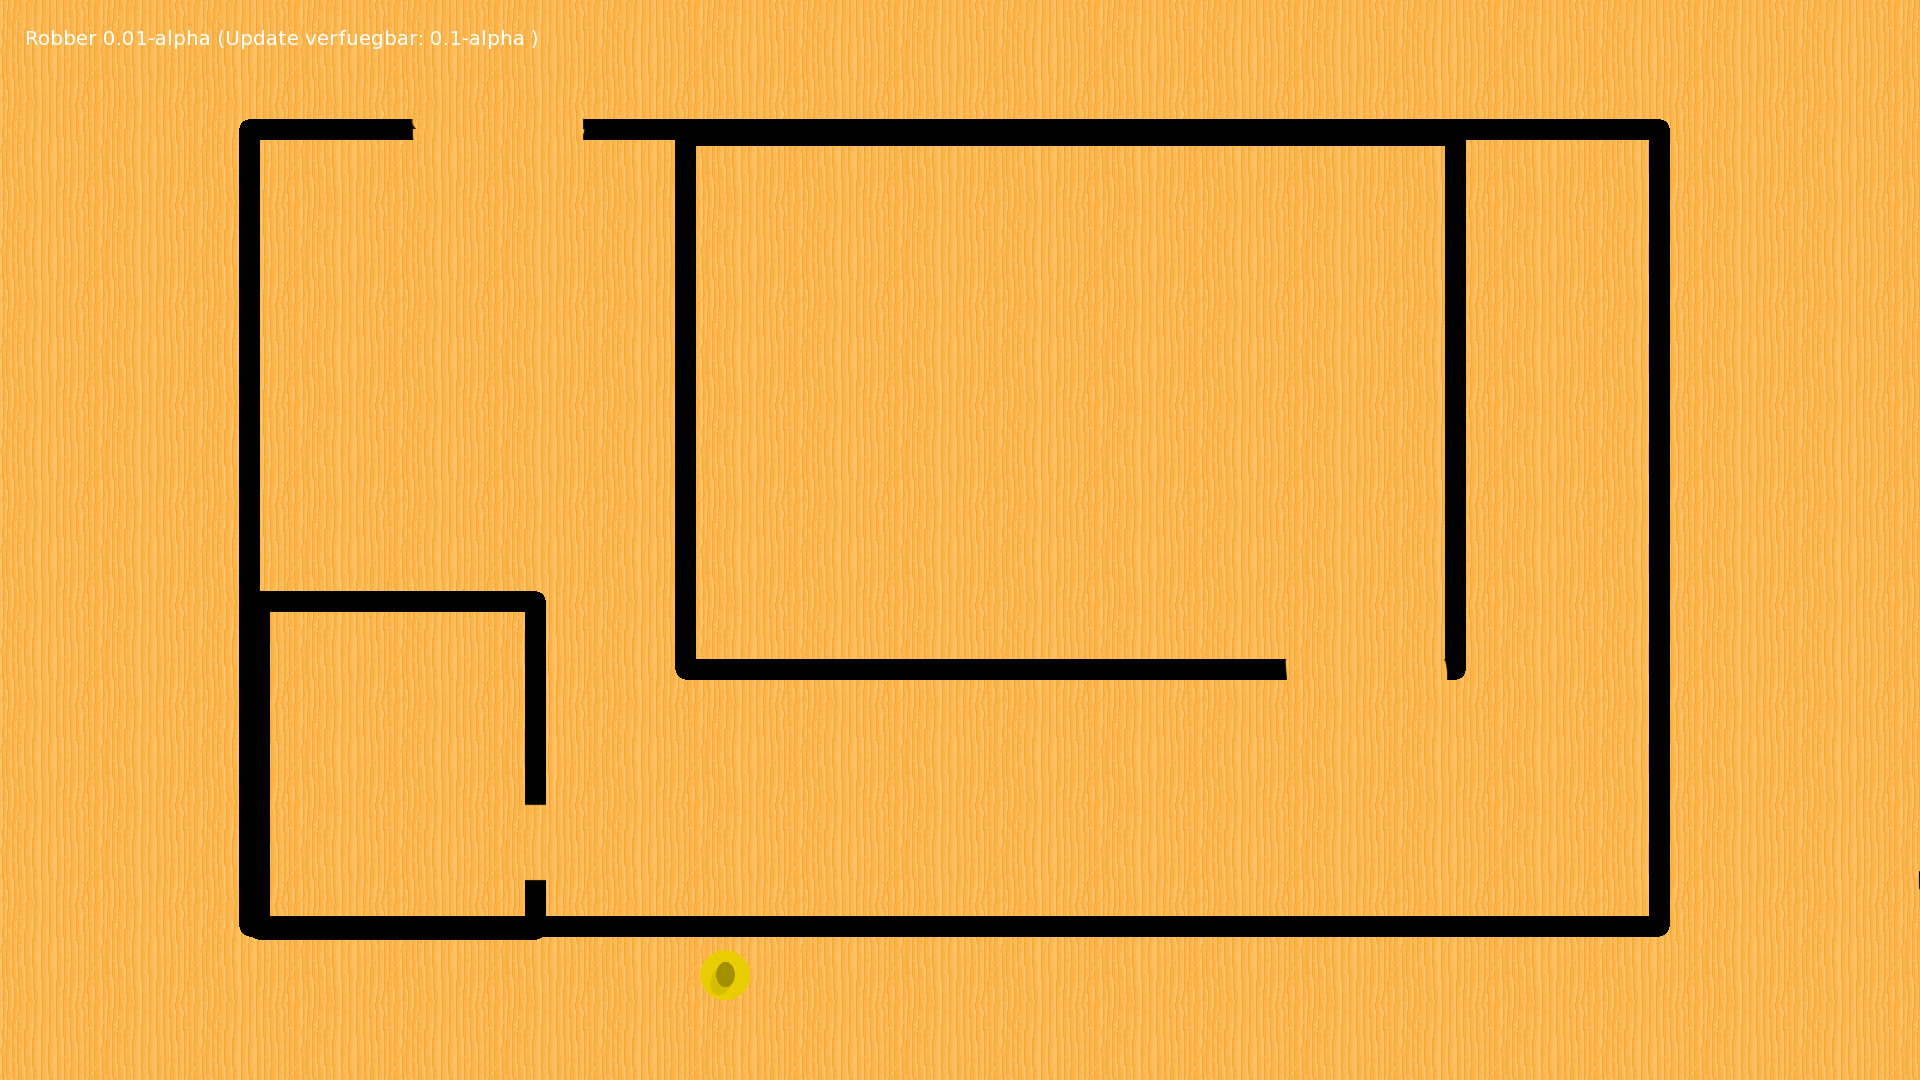
\includegraphics[scale=0.25]{img/grafiken.png}
\caption{Ein Beispiellevel mit der Spielfigur}
\end{figure}

\subsection{Kollisionsdetektion}
Die Kollisionsdetektion war zu Beginn der Entwicklungen etwas fehleranfällig. So gab es vereinzelt
Schlupflöcher ganz geringer Breite, sodass man durch die Mauer wandern konnte. Neben der Mauer hingegen,
versteckte sich eine unsichtbare Mauer, das heisst, es wurde eine Kollision gemeldet, obwohl an der
Spielerposition gar keine Mauer lag. Um das Problem zu Erforschen und schliesslich zu beheben, haben
wir die Mauerabschnitte einzeln geladen und ein grünes Rechteck darübergezeichnet. So fiel uns auf, dass
die Koordinaten der Mauer zwar richtig gelesen, aber falsch verarbeitet wurden. Die Koordinaten mussten
von absoluten Bildschirmkoordinaten in Fenster/Spielkoordinaten umgerechnet werden.

\begin{figure}[h]
\centering
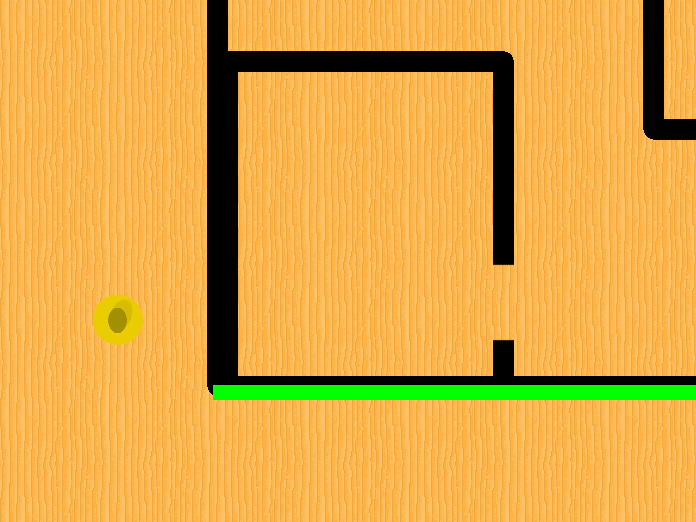
\includegraphics[scale=0.3]{img/kollisionsdetektion.png}
\caption{Debugging der Kollisionsdetektion}
\end{figure}

\subsection{Animationen}
Von Anfang an waren auch Animationen in unserem Spiel eingeplant. So sollen zum Beispiel ausserhalb eines Hauses
Türen durch grün blinkende/aufleuchtende Pfeile markiert werden. Für solche Animationen wurde eigens eine Klasse
implementiert.
\begin{figure}[h]
	\centering
	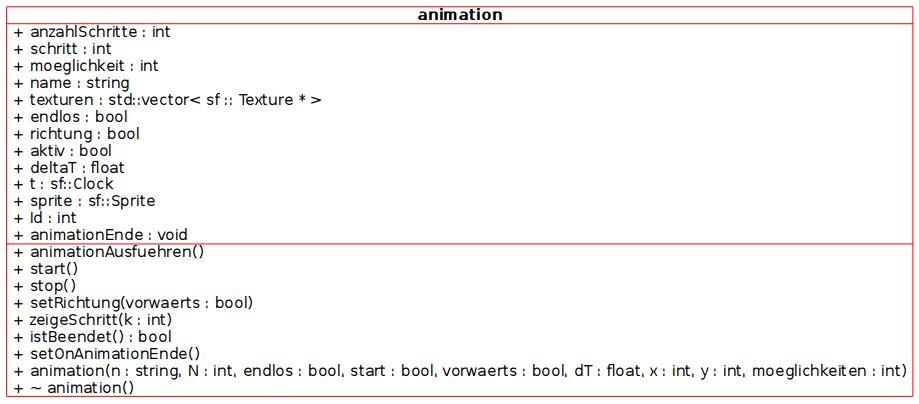
\includegraphics[scale=0.3]{img/animation_uml.png}
	\caption{UML: Animationsklasse}
\end{figure}
Um Animationen später oft und möglichst einfach verwenden zu können, besitzt die Klasse einen einfachen Konstruktor,
der die Bilder bereits lädt, die Position und die Zeitspanne $\Delta t$ zwischen den einzelnen Bildern festlegt.
\begin{figure}[h]
	\centering
	
\includegraphics[scale=0.3]{img/animation_pfeil.png}
	\caption{Die erste Animation im Spiel: Ein blinkender Einstiegspfeil}
\end{figure}
Innerhalb unserer $main()$-Funktion nützten wir eine $std::list<animation *>$ Liste aus der STL\footnote{Standard Template Library}.
Bevor die Sprites in das Fenster gezeichnet werden, werden die Texturen der Sprites dem Animationszeitpunkt entsprechend
neu geladen. So entsteht das Gefühl einer Bewegung, bzw. hier Anpassung der Farbe. Entscheidend ist dabei die Methode
$animationAusfuehren()$, die überprüft, ob bereits genug Zeit vergangen ist, das neue Bild anzuzeigen und dies gegebenenfalls
übernimmt.

\newpage
\listoffigures
\end{document}
